\providecommand{\main}{../..}
\documentclass[\main/notes.tex]{subfiles}

\begin{document}
	\setcounter{chapter}{6}
	\chapter{Operational Systems}
		\section{Enterprise Resource Planning}
			\begin{definition}{Enterprise Resource Planning (ERP)}
				A system that manages an entire company's vital business information.

				Evolved from \concept{material requirements planning (MRP)}, which allowed companies to plan out how much raw material they would need at a certain time in the future, plan their production, control their inventory, and manage their purchasing process.
			\end{definition}
			\begin{sidenote}{Advantages of ERP Systems}
				\begin{description}
					\item[Improved Access to Data for Operational Decision-Making] ERP systems use an integrated database -- use one set of data to support all business functions.
					\item[Elimination of Costly, Inflexible Legacy Systems] Replace separate systems with one, single, integrated system for the entire enterprise.
					\item[Improvement of Work Processes] As ERP development is designed to support best practices, this ensures the processes are based on these.
					\item[Upgrade of Technology Infrastructure] An organisation can eliminate the multiple hardware platforms, operating systems, and databases it is currently using. This reduces ongoing maintenance.
				\end{description}
			\end{sidenote}
			\pagebreak
			\begin{sidenote}{Disadvantages of ERP Systems}
				\begin{description}
					\item[Expense and Time in Implementation] Requires time and money in order to correctly set it up, and implement it
					\item[Difficulty Implementing Change] An organisation might require radical change in the way it operates in order to use the ERP System
					\item[Difficulty Integrating With Other Systems] Hard to integrate existing systems with a new ERP system
					\item[Difficulty in Loading Data into New ERP System] Need to load data from existing systems into the new one. This is dependent on the scope of ERP implementation.
						\begin{description}
							\item[Data mapping] The examination of each data item required for the new ERP system, and determining where the data item will come from. Often requires \concept{data clean-up} afterwards.
							\item[Data loading] Performed either by using data conversion software, or by end-users entering data via input screens of the new system.
						\end{description}
					\item[Risks in Using One Vendor] After an organisation has switched to a vendor for an ERP system, the vendor has less incentive to listen and respond to customer concerns.
					\item[Risk of Implementation Failure] Implementation requires large amounts of resources, the best IS and business people, and plenty of management support.
				\end{description}
			\end{sidenote}
			\subsection{ERP for Small- and Medium-Sized Enterprises (SMEs)}
				SMEs (both for-profit and not-for-profit) can achieve benefits using ERP. Many of these elect to use \concept{open-source ERP systems}, where the source code can be seen and modified.
				\begin{center}
					\begin{tblr}{colspec={cl}, row{1}={font=\bfseries}}
						\toprule
						Vendor & ERP Solutions\\
						\midrule
						Apache & Open For Business ERP\\
						Compiere & Compiere Open Source ERP\\
						Openbravo & Openbravo Open Source ERP\\
						WebERP & WebERP\\
						\bottomrule
					\end{tblr}
				\end{center}

		\pagebreak
		\section{Transaction Processing Systems}
			Examples of transaction processing systems (TPS):
			\begin{multicols}{2}
				\begin{itemize}[nosep]
					\item Order processing
					\item Inventory Control
					\item Payroll
					\item Accounts Payable
					\item Accounts Receivable
					\item General Ledger
				\end{itemize}
			\end{multicols}
			\begin{sidenote}{Transaction Processing System}
				\begin{description}[nosep]
					\item[Input] Basic Business Transactions
					\item[Processing] Data Collection, Data Editing, Data Correction, Data Manipulation, Data Storage, Document Production
					\item[Result] Organisation's records are updated to reflect the status of the operation at the time of the last processed transaction.
				\end{description}
				Also collects data which is input to other essential information systems, where it serves as a foundation of these other systems.

				Routine operations. The support for decision-making that is directly provided is \emph{low}.
			\end{sidenote}
			\subsection{Traditional Transaction Processing Methods and Objectives}
				\begin{definition}{Batch Processing Systems}
					A form of data processing where business transactions are accumulated over a period of time and prepared for processing as a single unit or batch.

					Some delay between an event and the eventual processing of the related transaction.

					Can be more cost-effective than OLTP.
				\end{definition}
				\begin{definition}{Online Transaction Processing (OLTP)}
					A form of data processing where each transaction is processed immediately, without the delay of accumulating transactions into a batch.

					The data in an online system reflects the current status.

					Can provide faster, more efficient service.
				\end{definition}
				\begin{sidenote}{Objectives of Transaction Processing Systems}
					\begin{itemize}[nosep]
						\item Process data generated by and about transactions
						\item Maintain a high degree of accuracy and integrity
						\item Avoid processing fraudulent transactions
						\item Produce timely user responses and reports
						\item Increase labour efficiency
						\item Help improve customer service
						\item Help build and maintain customer loyalty
						\item Achieve competitive advantage
					\end{itemize}
				\end{sidenote}
			\subsection{Transaction Processing Activities}
				\begin{definition}{Transaction Processing Cycle}
					The process of data collection, data editing, data correction, data manipulation, data storage, and document production.
					\begin{center}
						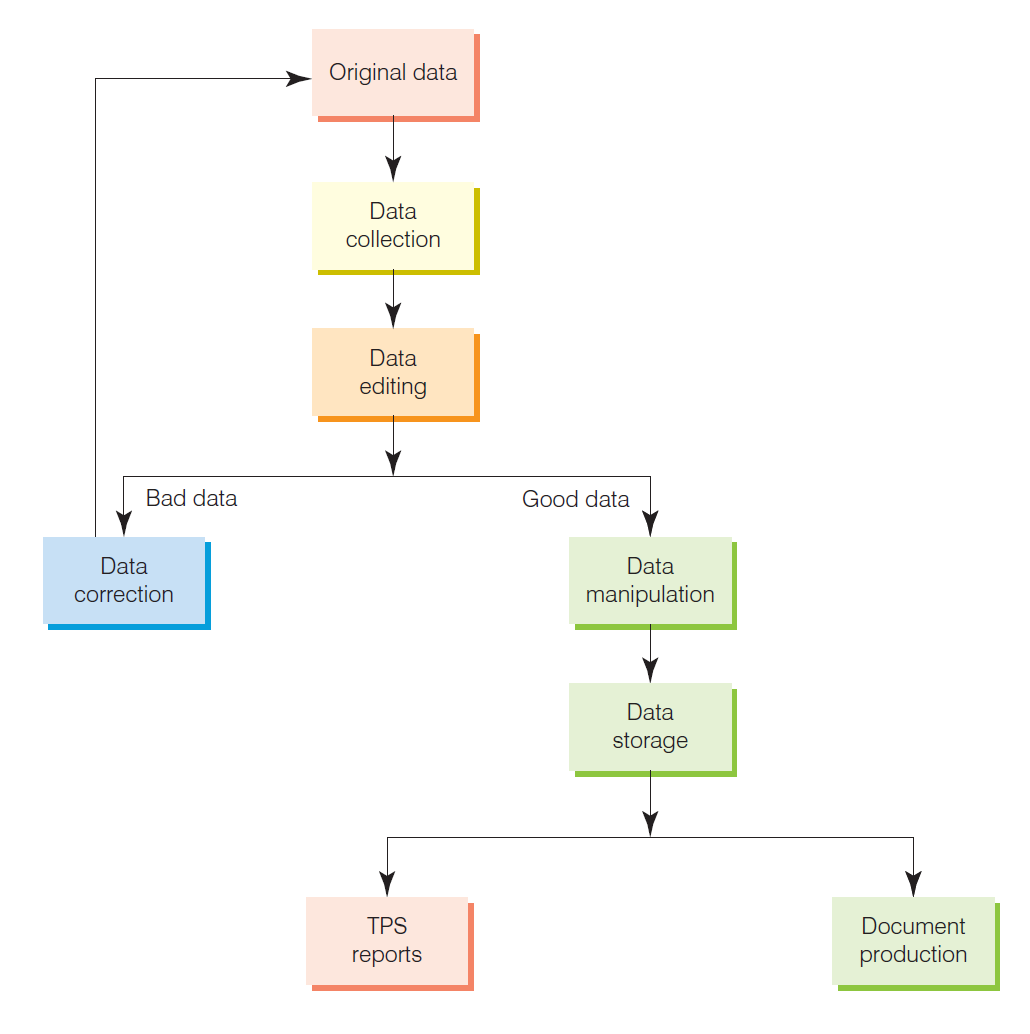
\includegraphics[width=0.75\textwidth]{chapter07/transaction_lifecycle.png}
					\end{center}
				\end{definition}
				\begin{definition}{Data Collection}
					Capturing and gathering all data necessary to complete the processing of transactions.

					Can be done manually, or automated using input devices such as barcode scanners and RFID readers. If done automatically, this is called \concept{source data automation}.

					Begins with a transaction and results in data that serves as input to the TPS.
				\end{definition}
				\begin{definition}{Data Editing}
					The process of checking data for validity and completeness.
				\end{definition}
				\begin{definition}{Data Correction}
					The process of re-entering data that was not typed or scanned properly.
				\end{definition}
				\begin{definition}{Data Manipulation}
					The process of performing calculations and other data transformations related to business transactions.
				\end{definition}
				\begin{definition}{Data Storage}
					Updating one or more databases with new transactions.
				\end{definition}
				\begin{definition}{Document Production}
					The process of generating output records and reports.
				\end{definition}

		\section{Traditional Transaction Processing Applications}
			\begin{sidenote}{Systems that support Order Processing, Purchasing, and Accounting Functions}
				\begin{tblr}{colspec={>{\raggedright}X>{\raggedright}X[2]>{\raggedright}X}, row{even}={bg={white}}, row{1}={font=\bfseries}}
					Order Processing & Purchasing & Accounting\\
					\midrule
					Order entry & Inventory control (raw materials, packing materials, spare parts, and supplies) & Budget\\
					Sales configuration & Purchase order processing & Accounts receivable\\
					Shipment planning & Receiving & Payroll\\
					Shipment execution & Accounts payable & Asset management\\
					Inventory control (finished product) & & General ledger\\
					Accounts receivable
				\end{tblr}
			\end{sidenote}
			\subsection{Order Processing Systems}
				\begin{tblr}[long]{colspec={>{\raggedright}X>{\raggedright}X[1.5]>{\raggedright}X[1.5]>{\raggedright}X}, row{even}={table even}, row{1}={font=\bfseries}, rowhead=1}
					\toprule
					System & Input & Processing & Output\\
					\midrule
					Order entry & Customer order information & Order checked for accuracy. On-hand inventory checked to ensure each item can be shipped, or a substitute item is suggested & An open order record\\
					Sales configuration & Customer order information & Review customer order information and ensure the configuration will meet customers needs. Suggest additional options and features & Revised customer order\\
					Shipment planning & Open orders & Determine which open orders will be filled, when, and from which location each order will be shipped & Pick list for each order, to be filled from each shipping location, showing the items and quantities needed\\
					Shipment execution & Pick list and data entered by warehouse operations personnel & Data entered by warehouse operations personnel captured and used to update record & A shipped order record specifying exactly what was shipped to the customer\\
					Inventory control (finished product) & Record of each item picked to fill a customer order & Inventory records updated to reflect current quantity of each item & Updated inventory database and various management reports\\
					Accounts receivable & Shipped order records, and payment from customers & Determine amount owed by each customer for each order placed & Invoice statement containing details for each order; customer's accounts receivable data is updated\\
					\bottomrule
				\end{tblr}
			\subsection{Purchasing Systems}
				\begin{tblr}[long]{colspec={>{\raggedright}X[1]>{\raggedright}X[2]>{\raggedright}X[2]>{\raggedright}X[2]}, row{even}={table even}, row{1}={font=\bfseries}}
					\toprule
					System & Input & Processing & Output\\
					\midrule
					Inventory control & Records reflecting any increase or decrease in the inventory of specific items of raw materials, packing materials, or spare parts & Withdrawals are subtracted from inventory counts, additions are added to inventory counts & The inventory record of each item is updated\\
					Purchase order processing & Inventory records, employee-prepared purchase order requests, information on preferred suppliers & Items and quantities that need to be ordered are determined, supplier is identified & Purchase order placed with preferred suppliers\\
					Receiving & Information on the quantity and quality of items received & Receipt matched to purchase order, input data is edited for accuracy and completeness & Receiving report is created, inventory records are updated\\
					Accounts payable & Purchase orders placed, information of receipts, supplier invoices & Supplier invoice matched to original purchase order and receiving report & Payment generated to supplier\\
					\bottomrule
				\end{tblr}
			\subsection{Accounting Systems}
				\begin{tblr}[long]{colspec={>{\raggedright}X[1]>{\raggedright}X[2]>{\raggedright}X[2]>{\raggedright}X[2]}, row{even}={table even}, row{1}={font=\bfseries}}
					\toprule
					System & Input & Processing & Output\\
					\midrule
					Budget & Amounts budgeted for various categories of expense & Accumulate amount spent in each budget category & Budget status report\\
					Accounts receivable & Shipment records specifying what was shipped to a customer & Determine amounts to be paid by customer, including delivery costs and taxes & Customer bills and monthly statements; management reports summarising customer payments\\
					Accounts payable & Purchase orders placed; information on receipts; supplier invoices & Supplier invoice matched to original purchase order and receiving report & Payment generated to supplier \\
					Payroll & Number of hours worked by employees; employee pay rate; employee tax and withholding information & Calculate employee gross and net pay, and amount to be withheld for statutory purposes and employee benefit programmes & Payment and payslip;payroll register\\
					Asset management & Data regarding the purchase of capital assets & Calculate depreciation and net value of all corporate assets & Listing of all assets, showing purchase price, and current value after depreciation\\
					General ledger & All transactions affecting the financial standing of the firm & Posts financial transactions to appropriate accounts specified & Financial reports; balance sheet\\
					\bottomrule
				\end{tblr}

		\section{Electronic and Mobile Commerce}
			\subsection{Electronic Commerce}
				\begin{definition}{Electronic Commerce (e-commerce)}
					Conducting a business transaction electronically over computer networks, such as the Internet, extranets and corporate networks.

					Can be thought of as a type of transaction processing system.
				\end{definition}
				\begin{definition}{Business to Consumer e-commerce (B2C)}
					A form of e-commerce in which customers deal directly with an organisation and avoid intermediaries.
					\begin{description}
						\item[Disintermediation] The elimination of intermediate organisations between the producer and the consumer.
					\end{description}
				\end{definition}
				\begin{definition}{B2Me e-ommerce}
					A form of e-commerce where the business treats each customer as a separate market segment.

					Typical B2Me features include customising a website for each customer, based on their previous purchases and personalised marketing literature.
				\end{definition}
				\begin{definition}{Business to Business e-commerce (B2B)}
					A subset of e-commerce where all the participants are organisations.

					Connect business partners in a virtual supply chain to cut re-supply times, and reduce costs.
				\end{definition}
				\begin{definition}{Consumer to Consumer e-commerce (C2C)}
					A subset of e-commerce that involves consumers selling directly to other consumers.
				\end{definition}
				\begin{definition}{E-government}
					The use of information and communications technology to simplify the sharing of information, speed up formerly paper-based processes and improve the relationship between citizen and government.
					\begin{description}
						\item[Government to Consumer (G2C)] Communicate directly between government and citizen. For example, tax returns and e-petitions.
						\item[Government to Business (G2B)] Communication between government and private businesses. Examples would be government purchasing materials and services from industry, and helping businesses receive current government regulations.
						\item[Government to Government (G2G)] Improve communications between the various levels of government. 
					\end{description}
				\end{definition}
			\subsection{Mobile Commerce}
				\begin{definition}{Mobile Commerce (m-commerce)}
					Relies on the use of wireless devices (such as personal digital assistants, mobile phones, and smartphones) to transact.

					To work effectively, the interface between the wireless device and its user needs to improve to the point that it is nearly as easy to purchase an item on a wireless device as it is to purchase on a home computer. Also, the network speed must improve to prevent user frustration.

					\concept{Security} is important:
					\begin{indentparagraph}
						\begin{description}[nosep]
							\item[Security of the transmission itself] Can be protected and assured using \concept{encryption}.
							\item[Transaction made with the intended party] Can be ensured using \concept{digital certificates}.
						\end{description}
					\end{indentparagraph}
				\end{definition}
				\begin{sidenote}{Limitations}
					\begin{itemize}[nosep]
						\item Small screens, so limited text
						\item Limited input capabilities, can be error-prone
						\item Less processing power and bandwidth
						\item Limited-life batteries
					\end{itemize}
				\end{sidenote}

		\section{Production and Supply Chain Management}
			\begin{description}[nosep]
				\item[1. Sales forecasting] Develop an estimate of future customer demand. At a fairly high-level with estimates made by product group.
				\item[2. Sales and Operations Plan] Consider demand and current inventory levels, and determine the specific product items that need to be produced and when to meet the forecast future demand.
				\item[3. Demand Management] Refine the production plan by determining the amount of weekly or daily production needed. The output is the \concept{master production schedule}, a production plan for all finished goods.
				\item[4. Detailed Scheduling] Use the production plan to develop a detailed production schedule specifying production scheduling details. A key decision is how long to make the production runs for each product.
				\item[5. Materials Requirement Planning] Determines the amount and timing for placing raw material orders with suppliers. Based on existing raw material inventory and the \concept{bill of materials (BOM)}, a list of materials needed to make each product. Depends on \concept{lead time}, the time it takes from when a purchase order is placed until the raw materials arrive; and \concept{lot size}, the discrete quantities that the supplier will ship, and the amount that is economical for the producer to receive and store.
				\item[6. Purchasing] Use the information from Materials Requirement Planning to place purchase orders for raw materials and transmit them to qualified suppliers.
				\item[7. Production] Use the detailed schedule to plan the details of running and staffing the production operation.
				\item[8. Capture information about production] Determine what was produced, and in what quantities. Can be done using personal computers that scan a \concept{universal product code (UPC)} on the packing material, or using RFID chips, or manually entering information. Separately, production quality can be measured, which typically uses the \concept{batch identification number}.
			\end{description}

		\section[Customer Relationship Management]{Customer Relationship Management and Sales Ordering}
			\subsection{Customer Relationship Management}
				\begin{definition}{Customer Relationship Management (CRM) System}
					A system that helps a company manage all aspects of customer encounters, including marketing and advertising, sales, customer service after the sale, and programmes to retain loyal customers.

					The goal is to understand and anticipate the needs of current and potential customers, to increase customer retention and loyalty, while optimising the way that products and services are sold.
					\begin{center}
						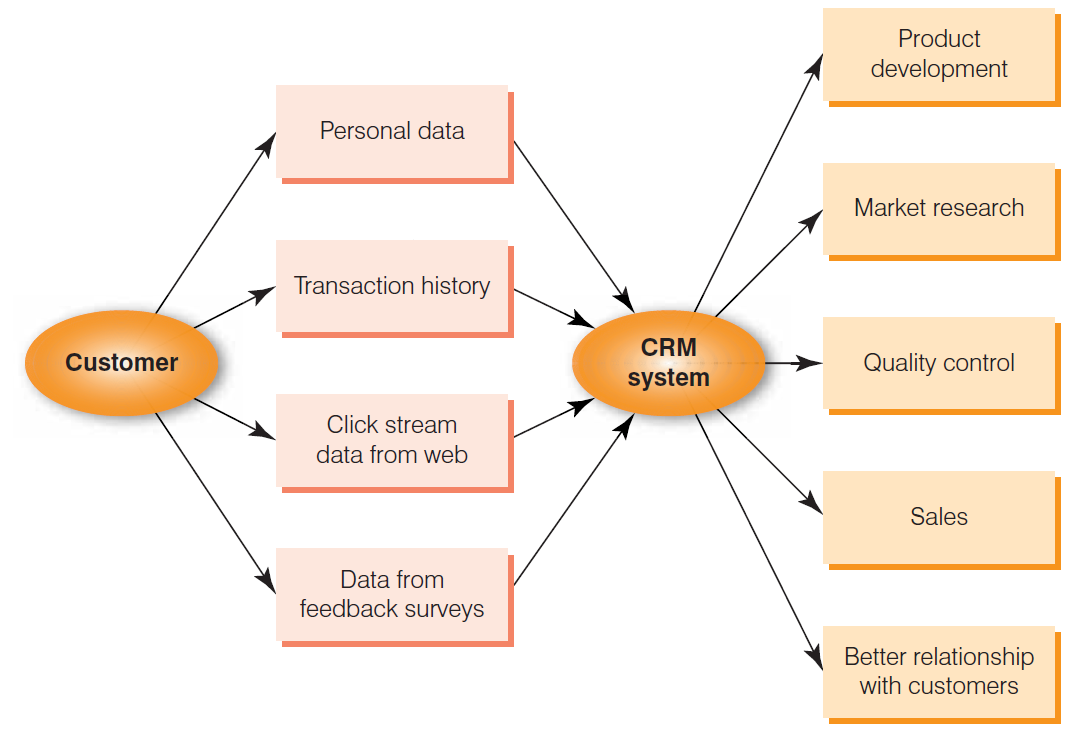
\includegraphics[width=0.75\textwidth]{chapter07/customer_relationship.png}
					\end{center}
				\end{definition}
			\subsection{Sales Ordering}
				\begin{definition}{Sales Ordering}
					The set of activities that must be performed to capture a customer sales order. Includes recording the times to be purchased, setting the sales price, recording the order quantity, determining the total cost of the order including delivery costs, and confirming the customer's available credit.
				\end{definition}

		\pagebreak
		\section{Financial and Managerial Accounting}
			\begin{definition}{General Ledger}
				The main accounting record of a business. Often divided into different categories, including:
				\begin{multicols}{2}
					\begin{itemize}[nosep]
						\item assets
						\item liabilities
						\item revenue
						\item expenses
						\item equity
					\end{itemize}
				\end{multicols}
				These categories are then further subdivided into sub-ledgers:
				\begin{multicols}{2}
					\begin{itemize}[nosep]
						\item cash
						\item accounts payable
						\item accounts receivable
						\item etc.
					\end{itemize}
				\end{multicols}
			\end{definition}
			\begin{definition}{Financial Accounting}
				Capturing and recording all the transactions that affect a company's financial state, and then using these documented transactions to prepare financial statements for external decision-makers.
			\end{definition}
			\begin{sidenote}{Hosted Software Model for Enterprise Software}
				A pay-as-you-go approach that appeals to small businesses, as they can experiment with powerful software capabilities without making a major financial investment.
			\end{sidenote}

		\section{International Issues Associated with Operational Systems}
			\begin{sidenote}{International Issues}
				\begin{itemize}
					\item Different Languages and Cultures
					\item Disparities in IS infrastructure
					\item Varying laws and customs
					\item Multiple currencies
				\end{itemize}
			\end{sidenote}
	\vbox{\rulechapterend}
\end{document}